\documentclass{article}
\usepackage[utf8]{inputenc}
\usepackage[a4paper, margin=2.5cm]{geometry}
\usepackage{graphicx}
\usepackage[french]{babel}

\usepackage[default,scale=0.95]{opensans}
\usepackage[T1]{fontenc}
\usepackage{amssymb} %math
\usepackage{amsmath}
\usepackage{amsthm}
\usepackage{systeme}

\usepackage{hyperref}
\hypersetup{
    colorlinks=true,
    linkcolor=blue,
    filecolor=magenta,      
    urlcolor=cyan,
    pdftitle={SIGNAL},
    % pdfpagemode=FullScreen,
    }
\urlstyle{same} %\href{url}{Text}

\theoremstyle{plain}% default
\newtheorem{thm}{Théorème}[section]
\newtheorem{lem}[thm]{Lemme}
\newtheorem{prop}[thm]{Propriété}
\newtheorem*{cor}{Corollaire}
%\newtheorem*{KL}{Klein’s Lemma}

\theoremstyle{definition}
\newtheorem{defn}{Définition}[section]
\newtheorem{exmp}{Exemple}[section]
\newtheorem{xca}[exmp]{Exercise}

\theoremstyle{remark}
\newtheorem*{rem}{Remarque}
\newtheorem*{note}{Note}
%\newtheorem{case}{Case}



\title{Traitement du signal}
\author{Charles Vin}
\date{2022}

\begin{document}
\maketitle

Cours de \begin{itemize}
    \item Hassam Aboushady, équipe CIAN : hassam.aboushady@lip6.fr. Cours inspiré des 5 premiers chapitre du livre "B.P.Lathi, Linear Signals \& Systems, Oxford University Press 2005" 
    \item Sebastien Baey : sebastien.baey@lip6.fr
\end{itemize}

Modalité d'examen : 
\begin{itemize}
    \item Un exam par professeur après chaque partie. 
    \item Pour Aboushady : 60\% exam, 40\% sur les CR de TD chaque semaine into 50\% de la note finale + une feuille A4
    \item Pour Baey à voir
\end{itemize}

Table des matières 
\begin{itemize}
    \item Signaux et opération utiles
    \item Traitement de signal dans le domaine Temporel (convolution) \begin{itemize}
        \item Temps continu
        \item Temps discret
    \end{itemize}
    \item Traitement de signal dans le domaine fréquentiel \begin{itemize}
        \item Transformé de Laplace (Temps continu)
        \item Transformé en Z (Temps discret)
    \end{itemize}
    \item Filtrage en temps continu/discret
\end{itemize}

Quatres type de signal : Temps continu/discret X Amplitude Analogique(continue)/numérique(discret). D'un point de vu technique, le type d'amplitude ne change pas grand chose (ça rajoute juste une erreur qu'on modélise comme du bruit). Ce qui est important est le type de temps.

\tableofcontents

\section{Opération sur les signaux}
\subsection{Quelques révisions}
On a \begin{itemize}
    \item Un signal $ x(t) $ en entrée
    \item Qui passe dans un système $ h(t) $ 
    \item Qui sort un autre signal $ y(t) $ 
\end{itemize}
3 opérations : Voir les graphique dans OneNote
\begin{itemize}
    \item Décalage : On décale le signal dans le temps $ x(t+T), x(t-T)$ 
    \item Etalage et compression dans le temps : \begin{itemize}
        \item Etalage : $ x(t/2) $ Aplatie la courbe dans le temps 
        \item Compression : $ x(2t) $ L'inverse
    \end{itemize}
    \item Inversion : $ x(-t) $ : symétrie par rapport à l'ordonnée. 
\end{itemize}

On vas écrire les fonctions de signal en utilisant cette fonction
\[
    \begin{cases}
        1 &\text{si } t \leq 0\\
        0 &\text{si } t > 0\\
    \end{cases} 
.\]
\begin{exmp}[]
    Exprimer $ x(t) $ en fonction de $ u(t) $. Voir OneNote
\end{exmp}

\begin{defn}[L'impulsion (dirac)]
    On mesure l'impulsion (le saut si on prend une porte) avec cette fonction. L'amplitude ici est infini ( mot du prof mais genre la pente est infini). 
    \[
        \delta (t) = 0 \text{ pour } t \neq 0 , \int_{- \infty }^{\infty } \delta (t) dt = 1
    .\]
    En faite il le mesure avec cette fonction mais il a fait un dessin où il fait tendre $ \epsilon \to 0 $ pour reserrer la fenêtre de l'intégrale autour de la porte 
\end{defn}

\begin{defn}[L'exponentiel]
    On passe dans les complexes où on écrit le nombre imaginaire avec $ i $ ou $ j $ (pour pas confondre le $ i $ de l'intensité du courant). \begin{align*}
        e^{st} \text{ avec } s &= a + jb \\
        e^{st} = e^{(a+jb)t} &= e^{at} e^{jbt} \\
                            &= e^{at}(\cos (bt) + j \sin bt)
    \end{align*}
\end{defn}

\subsection{La convolution}
\begin{defn}[]
    En gardant en tête la définition de tout à l'heure avec le signal d'entrée $ x(t) $ et le système $ h(t) $. On définie l'intégrale de la convolution tel que 
    \begin{align*}
        y(t) = x(t) \star h(x) &= \int_{-\infty}^{\infty } x(\tau  )h(t-\tau  ) d \tau  \\
        & = \int_{-\infty }^{\infty }h(\tau  )x(t-\tau    d \tau  )
    \end{align*}
\end{defn}
\begin{exmp}[]
    Déterminez la réponse d'un système définit par $ h(t) = e^{-2t} u(t)$  à une entrée $ x(t)=e^{-t}u(t) \to u(\tau ) $. 
    \begin{align*}
        y(t) = x(t) \star h(t) &= \int_{(\infty )}^{\infty } x(\tau )h(t-\tau )d \tau \\
        &= \int_{0}^{t}e^{-\tau }e^{-2(t-\tau )}d \tau 
    \end{align*}
    Voir figure \ref{exmp_conv_1}.
    \begin{figure}[!htbp]
        \centering
        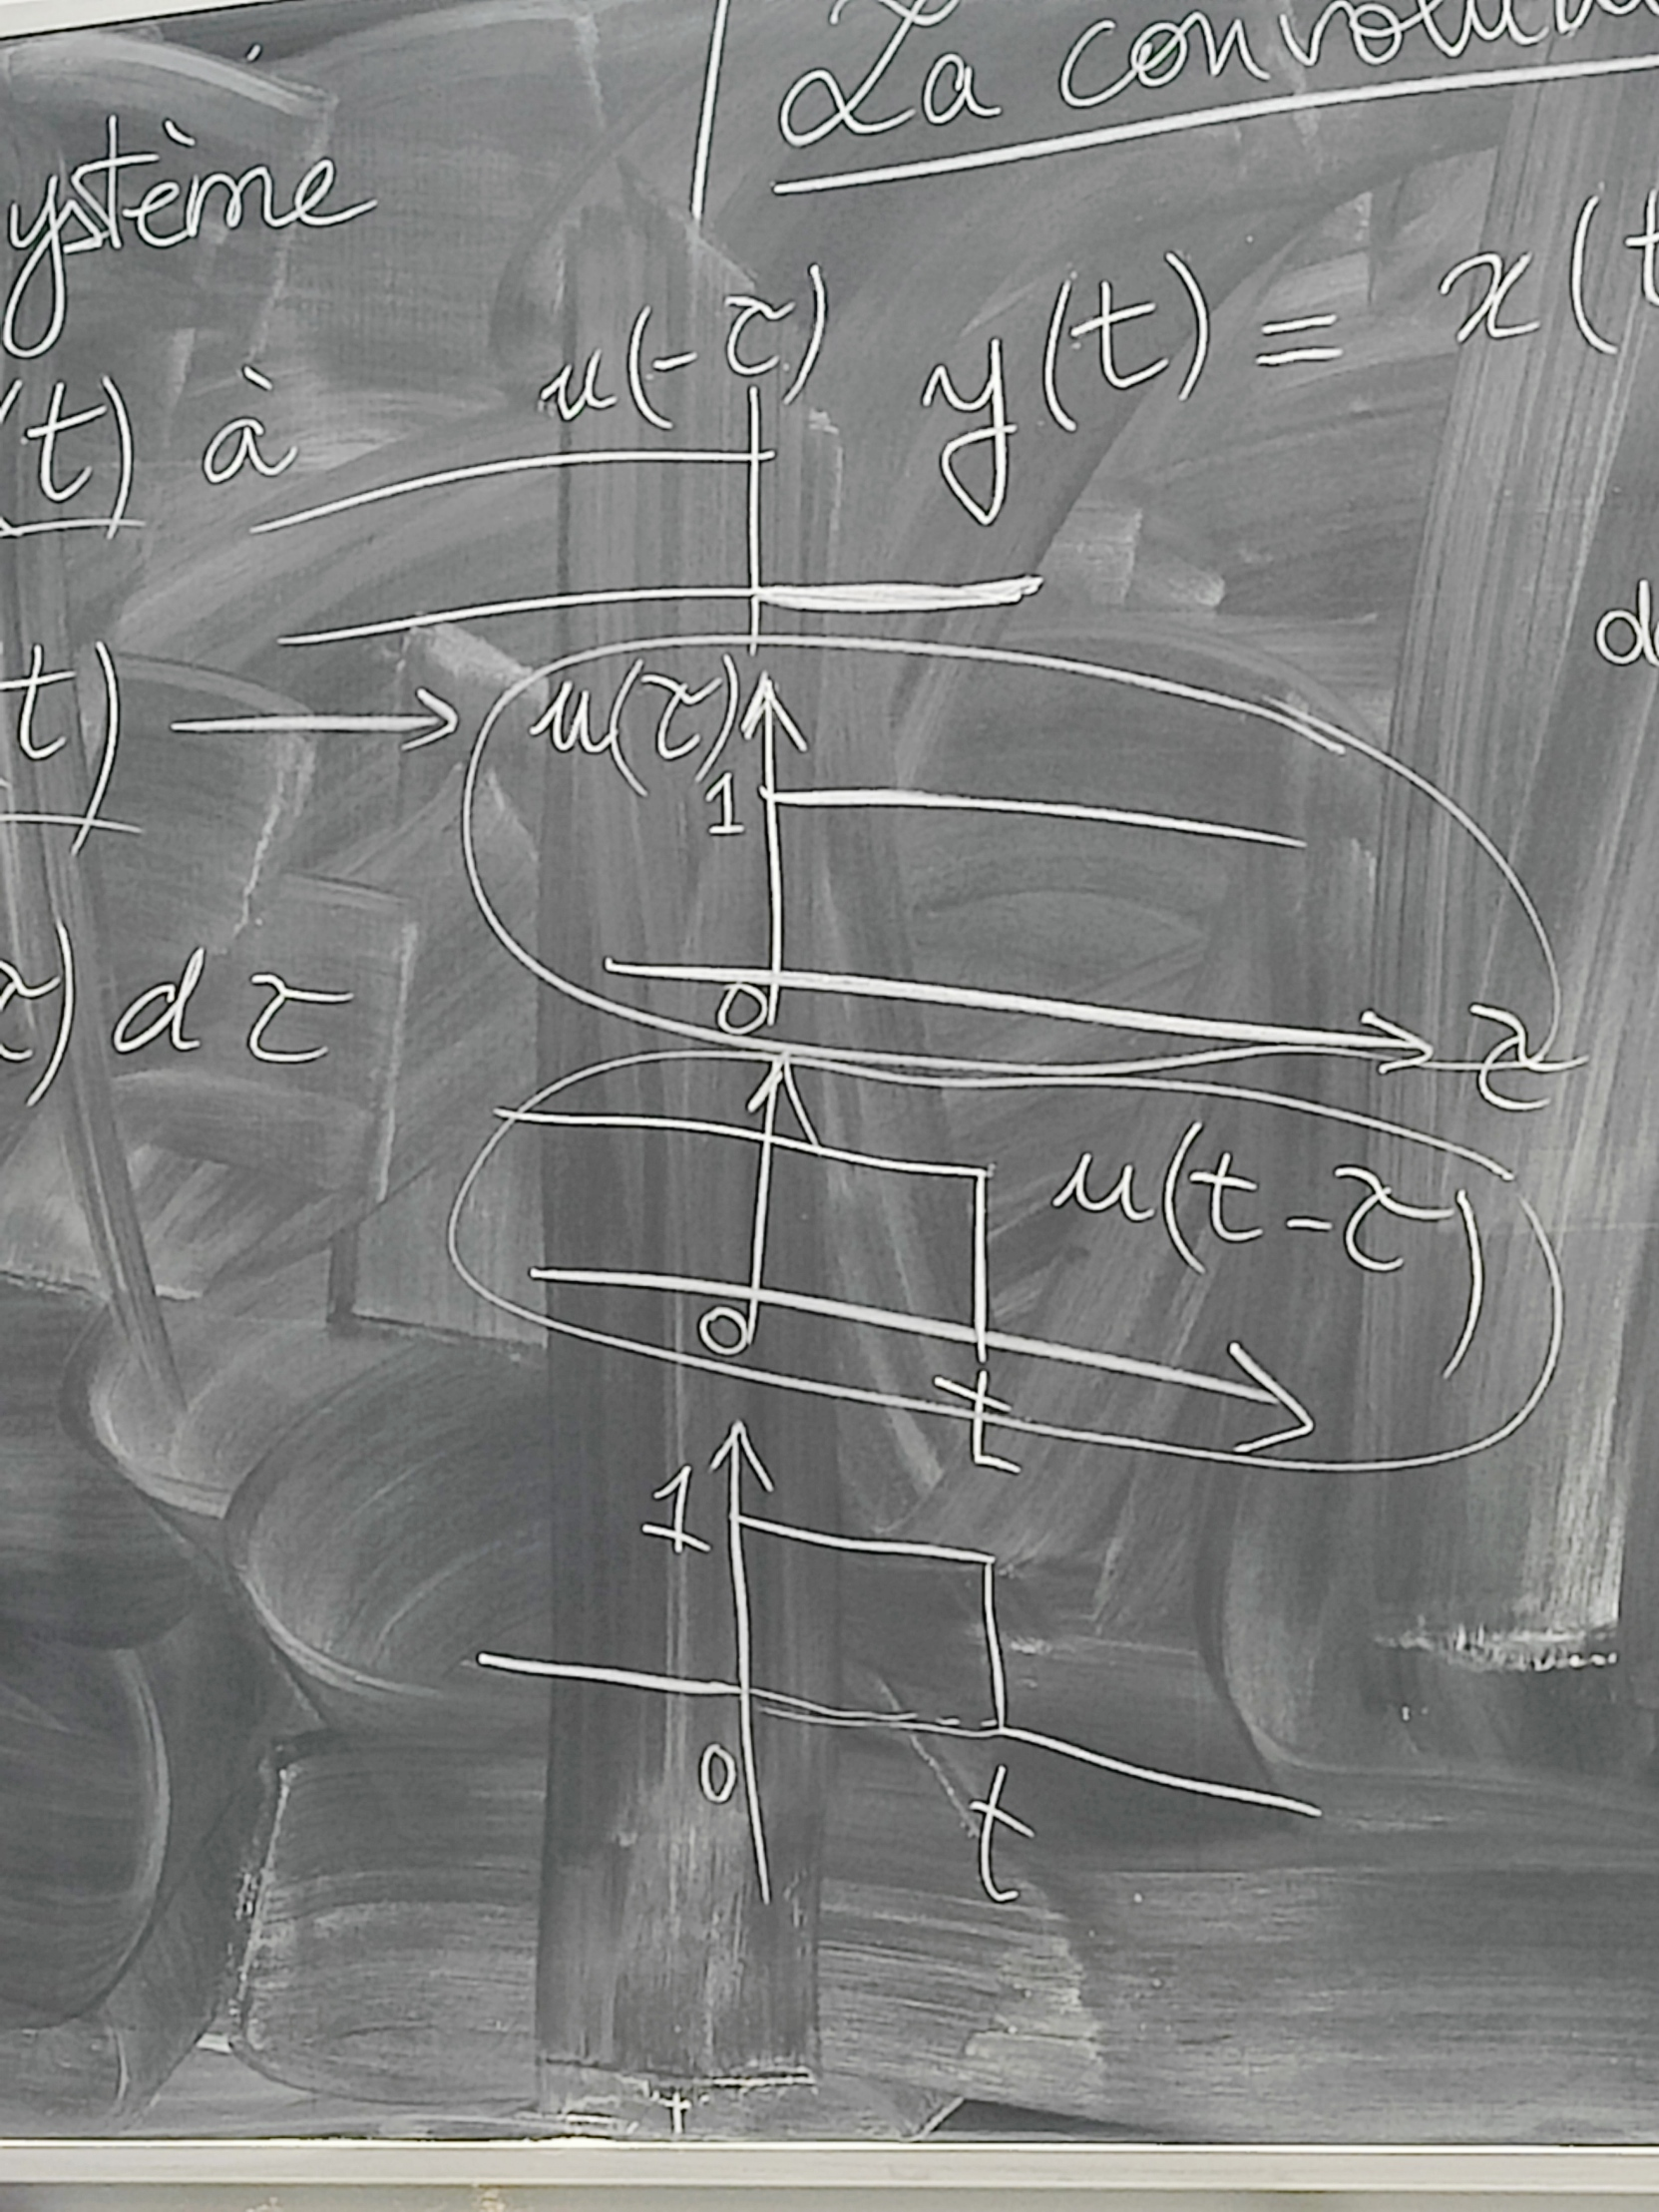
\includegraphics[width=.60\textwidth]{./figures/fig1.jpg}
        \caption{Exemple convolution}
        \label{exmp_conv_1}
    \end{figure}
\end{exmp}
\begin{prop}[de la convolution]
    Quelques propriété de la convolution
    \begin{itemize}
        \item Commutativité : $ x_1(t) \star x_2(t) = x_2(t) \star x_1(t) $ 
        \item Distributivité : toi même tu sais
        \item Associativité : $ x_1(t) \star x_2(t) \star x_3(t) = (x_1(t) \star x_2(t)) x_3(t) = x_1(t) \star (x_2(t) \star x_3(t)) $ 
        \item Décalage : Si $ x_1(t) \star x_2(t) = c(t) $ alors \begin{align*}
            x_1(t) &\star x_2(t-T) = c(t-T) \\
            x_1(t-T) &\star x_2(t) = c(t-T) \\
            x_1(t-T_1) &\star x_2(t-T_2) = c(t-T_1 - T_2) \\
        \end{align*}
        \item Convolution avec une impulsion : $ x(t) \star \delta (t) = x(t) $ 
        \item La durée de la convolution : On somme les deux durées (temps entre le zéro du début et celui de la fin). Soit un signal $ x_1(t) $ d'une durée $ T_1 $ et un signal $ x_2(t) $ d'une durée $ T_2 $. Alors $ x_1(t) \star x_2(t) $ à une durée de $ T_1 + T_2 $. 
    \end{itemize}
\end{prop}

\subsubsection{La convolution graphique de $ x(t) \star h(t) $ }
\begin{enumerate}
    \item Je garde $ x(\tau ) $ fixe (ou $ h(t) $ )
    \item Je trace $ h(-\tau ) $ (ou $ x(t) $ )
    \item Je décale $ h(-\tau ) $ pour une valeur de $ t $ (ou $ x(t) $ )
    \item J'intègre $ x(\tau )h(t -\tau ) $ dans chaque cas (ou inverses)
    \item Je répète 3. et 4. pour différentes valeurs de $ t $ 
\end{enumerate}
\begin{exmp}[]
    Trouvez la convolution de $ x(t), h(t) $. Voir one note
\end{exmp}

\underline{Nouveau \textbf{TP1} du 22/09} \\

\begin{defn}[Parité]
    Fonction paire et impaire 
    \begin{itemize}
        \item si $ x(t) = x(-t) $ $\rightarrow$ fonction paire
        \item si $ x(t) = -x(t) $ $\rightarrow$ fonction impaire
    \end{itemize}
    On peut écrire une fonction $ x(t) $ de ses composantes paire et impaire.
    \[
        x(t) = \frac{1}{2}(x(t) + x(-t)) + \frac{1}{2}(x(t) - x(-t))
    .\]
\end{defn}


\begin{xca}[1]
    Écrivez $ x(t) = e^{-at}u(t)$ en fonction de ses composantes paires et impaires. \begin{itemize}
        \item La fonction paire $ x_p(t) = \frac{1}{2}(x(t) + x(-t)) $ 
        \item La fonction impaire $ \frac{1}{2} (x(t) - x(-t)) $ 
    \end{itemize}
    Dessin dans OneNote.
\end{xca}

\section{Système linéaire et invariant dans le temps}
\begin{defn}[Système linéaire et invariant dans le temps]
    Le système doit être \textbf{additif}, \textbf{homogène} et \textbf{invariant dans le temps}. \begin{itemize}
        \item Additif : Si $ y_1(t) = y_2(t) $ donc le système $ h(t) $ est additif.
        \item Homogène : Si $ y_1(t) = y_2(t) $ donc le système $ h(t) $ est homogène.
        \item Invariant dans le temps : Si $ y_1(t) = y_2(t) $ donc le système est invariant dans le temps.
        \item Voir dessin Onenote
    \end{itemize}
\end{defn}

\begin{xca}[2]
    Trouvez si les systèmes suivant sont linéaire et invariant dans le temps.\begin{align}
        y(t) = x(t)\cos(2 \pi ft)\\
        y(t) = sin(x(t))
    \end{align}
    Réponse dans OneNote
\end{xca}

\begin{xca}[]
    Trouver le résultat de la convolution $ x(t) \star h(t) $ \begin{align*}
        x(t) &= u(t) - u(t-4) \\
        h(t) &= tu(t)
    \end{align*}
    Correction dans OneNote : \begin{align*}
        x(t) &= \int_{-\infty }^{\infty } x(\tau )h(t-\tau )d \tau \\
            &= \int_{-\infty }^{\infty } h(\tau )x(t-\tau )d \tau
    \end{align*}
\end{xca}

\begin{xca}[]
    Trouver le résultat de la convolution $ x(t) \star h(t) $ \begin{align*}
        x(t) &= u(t) - u(t-4) \\
        h(t) &= tu(t)
    \end{align*}
    Correction dans OneNote
\end{xca}

\begin{xca}[]
    Trouver le résultat de la convolution $ x(t) \star h(t) $ \begin{align*}
        x(t) &= \sin (t) [u(t) - u(t-2 \pi )] \\
        h(t) &= u(t-1) - u(t-3)
    \end{align*}
    Correction dans OneNote
\end{xca}

\paragraph*{A rendre sous forme de compte rendu avant le 28/09/2022}
\begin{xca}[]
    Trouver les composante paires et impaires de $ x(t) $: Dessin OneNote
\end{xca}
\begin{xca}[]
    Déterminez si les systèmes suivants sont linéaire et invariant dans le temps \begin{align}
        y(t) &= t^2 \frac{dx(t)}{dt} \\
        y(t) &= \cos (2 \pi ft + x(t))
    \end{align}
\end{xca}
\begin{xca}[]
    Trouver la convolution de $ x(t) $ et $ h(t) $ : 
    \begin{itemize}
        \item Dessin OneNote
        \begin{align*}
            x(t) &= 2 u(t-10) \\
            h(t) &= \sin (2t) u(t)
        \end{align*}
        \item \begin{align*}
            x(t) &= u(t) \\
            h(t) &=\text{ voir onenote}
        \end{align*}
        \item Voir OneNote
    \end{itemize}
\end{xca}
\begin{xca}[]
    Tracer avec MatLab les 3 courbes suivantes sur la même figure $ \forall t \in [0, 10] $ 
    \begin{align}
        w(t) &= e^{-t} \\
        x(t) &= te^{-t} \\
        y(t) &= e^{-t} + te^{-t}
    \end{align}
\end{xca}

\paragraph*{Intro MatLab}
Commande importante \begin{itemize}
    \item Size : check la size d'un vecteur 
    \item Length : Pareil pour les matrices
    \item Load/Save : Sauver des résultats
\end{itemize}
On évite $ i $ et $ j $ car dans MatLab c'est les variables complexes.\\
Faire attention au opérateur $ * $ = le produit scalaire et $ .* $  = le produit terme à terme de matrice.\\
Faire le graph de sin : \begin{align*}
    t &= 1:0.001:10 \\
    y &= sin(t) \\
    plot&(t,y) \\
    xlabel&('\text{Temps en seconde}') \\
    ylabel&('\text{Amplitude}')
\end{align*}
Log scale : $ semilogx(f, module) $, $ subplot $ pour subplot. \\
Plusieurs courbes : \begin{align*}
    x_1 &= e^{-t} \\
    x_2 &= t \\
    x_3 &= t + e^{-t} \\
    plot(t,x_1,'b', t,x_2,'r', t,x_3, 'g') \\
    c
\end{align*}



\underline{Nouveau cours du 23/09} \\

\subsection{La transformé de Laplace}
Dans le cas de la transformé de Laplace on a 
\[
    x(t) \rightarrow h(t) \rightarrow y(t)
.\]
qui devient
\[
    X(S) \rightarrow H(S) \rightarrow Y(S) = X(S)H(S)
.\]
\begin{defn}[La transformé de Laplace]
    \begin{align*}
        X(S) &= \mathcal{L}\{x(t)\} \\
            &= \int_{-\infty }^{\infty }x(t) e^{-St}dt
    \end{align*}
    avec $ S = \sigma + j \omega \text{ ( imaginaire )}, w = 2 \pi f, f=\text{ la frequence}$
\end{defn}
\begin{exmp}[Laplace]
    Ici on montre comment les valeurs du tableau poly sont calculées.
    \begin{align*}
        \mathcal{L}(u(t)) &= \int_{-\infty }^{\infty }u(t)e^{St}dt \\
            &= \int_{0}^{\infty }e^{-St}dt = [\frac{e^{St}}{-S}]^{\infty }_0 \\
            &= 0 - \frac{e^0}{-S} = \frac{1}{S}
    \end{align*}
\end{exmp}
\begin{exmp}[]
    Ici on montre comment les valeurs du tableau poly sont calculées.
    \begin{align*}
        \mathcal{L}\{\cos (\omega _0 t) u(t)\} &= \int_{-\infty }^{\infty }\cos (\omega _0 t) u(t)e^{St}dt \\
        &= \int_{0}^{\infty }\cos (\omega_0 t) e^{-St}dt \\
        &= \int_{0}^{\infty }(\frac{e^{j \omega _0 t } + e^{-j \omega_0 t }}{2}) e^{St} dt \\
        &= \frac{1}{2} \int_{0}^{\infty } e^{t(j\omega _0 - S)} + e^{-t(j \omega _0 + S)} dt \\
        &= \frac{1}{2} [\frac{e^{t(j \omega _0 - S)}}{j \omega_0 - S} - \frac{e^{-t(j \omega _0 + S)}}{j \omega_0 + S}]_{0}^{\infty } \\
        & \text{Ici y'a un problème de convergence avec le } + \infty \text{ le prof ne sais pas} \\
        &= \frac{1}{2} (\frac{0 - 1}{j \omega _0 - S} + \frac{0 - 1}{-(j \omega _0 + S)}) \\
        &= \frac{1}{2} (\frac{1}{S - j \omega _0} + \frac{1}{S + j \omega _0}) \\
        &= \frac{1}{2} (\frac{S + j \omega _0 + S - j \omega _0}{S^2 + \omega _0^2}) \\
        &= \frac{S}{S^2 + \omega _0 ^2}
    \end{align*}
\end{exmp}

\begin{prop}[importante de la transformé de Laplace]
    \begin{itemize}
        \item Addition : $ \mathcal{L}\{x_1(t) + x_2(t)\} = X_1(S) + X_2(S)$ 
        \item Dérivé (sous condition) : $ \mathcal{L}\{\frac{dx(t)}{dt}\} $ 
        \item Dérivé seconde : $ \mathcal{L}\{\frac{d^2x(t)}{dt^2}\} $ 
        \item Intégrale : $ \mathcal{L}\{\int_{0}^{t}x(t)dt\} = \frac{1}{S}X(S) $ 
        \item \textbf{Convolution} : $ \mathcal{L}\{x_1(t) \star x_2(t)\} = X_1(S) X_2(S)$ 
        \item Time shifting : $ \mathcal{L}\{x(t-t_0) u(t - t_0)\} = X(S)e^{-t_0 S}$ 
    \end{itemize}
\end{prop}

\subsection{Transformé de Laplace Inverse}

\begin{exmp}[Transformé de Laplace Inverse]
    Cas général avec décomposition en élément simple.
    \[
        H(S) = \frac{7S - 6}{S^2 - S - 6}
    .\]
    Racine du dénominateur : $ 3 $ et $ -2 $ $\rightarrow$ Factorisation du dénominateur en $ (S-3)(S+2) $ 
    \[
        \frac{7S-6}{(S-3)(S+2)} = \frac{A}{S+2} + \frac{B}{S+2}
    .\]
    Pour trouver $ A $ et $ B $ : \href{https://www.methodemaths.fr/decomposition_elements_simples/#principe}{Trois techniques} \begin{itemize}
        \item Par identification en remultipliant en haut et en bas 
        \item Multiplier par un des facteurs à gauche et à droite pour simplifier une des fractions, remplacer $ S $ par $ -2 $ pour obtenir $ -2+2 = 0 $, ça simplifie plein de truc et hop on peut retrouver $ B $ facilement.
        \item 
    \end{itemize}
    Bref ici $ A = 4 $ et $ B=3 $ \begin{align*}
        H(S) &= \frac{4}{S+2}  + \frac{3}{S - 3} \\
        \downarrow \mathcal{L}^{-1}& \\
            h(t) &= 4 e^{-2t} u(t) + 3 e^{3t} u(t)
    \end{align*}
\end{exmp}

\subsection{Expression générale d'un système linéaire invariant dans le temps}
\begin{align*}
    &\frac{d^N}{dt^N} y(t) + a_{N-1}\frac{d^N}{dt^N} y(t) + \dots + a_1 \frac{d}{dt}y(t) + a_0 y(t) \\
    =& b_M \frac{d^M x(t)}{dt^M} + b_{M-1} \frac{d^{M-1} x(t)}{dt^{M-1}} + \dots + b_1 \frac{d x(t)}{dt} + b_0 x(t)
\end{align*}
En supposant toutes les conditions initiales nulles et en appliquant la transformée de Laplace : 
\begin{align*}
    & [S^N + a_{N-1} S^{N-1} + \dots + a_1 S + a_0]Y(S) = [b_M S^M + b_{M-1} S^{M-1} + \dots + S b_1 + b_0] X(S) \\
    \Leftrightarrow & \frac{Y(S)}{X(S)} = \frac{b_M S^M + b_{M-1} S^{M-1} + \dots + S b_1 + b_0}{S^N + a_{N-1} S^{N-1} + \dots + a_1 S + a_0} \\ 
    \Leftrightarrow & H(S) = \frac{Y(S)}{X(S)} = \frac{(S + z_1) + (S + z_2) + \dots + (S + z_M)}{(S + p_1) + (S + p_2) + \dots + (S + p_N)}
\end{align*}
Avec $ H(S) $ la fonction de transfert, $ z_1, \dots, z_M $  les \textbf{zéros de la fonction de transfert} et $ p_1, \dots, p_N $ les \textbf{pôles de la fonction de transfert}.
\begin{align*}
    H(S) &= \frac{A}{S+p_1} + \frac{B}{S+p_2} + \dots + \frac{N}{S + p_N} \\
    \mathcal{L}^{-1} \downarrow & \\
    h(t) &= Ae^{-p_1t} + Be^{-p_2t} + \dots + Ne^{-p_Nt}
\end{align*}

\begin{exmp}[Stabilité d'un système LTI]
    \textbf{uniquement les pôles ont une influence sur la stabilité (?)}
    \begin{align*}
        H(S) &= \frac{1}{S+p_1} \rightarrow_{\mathcal{L}^{-1}} h(t) = e^{-p_1t} \\
            &= \frac{1}{s-p_1} \to_{\mathcal{L}^{-1}} h(t) = e^{p_1t}
    \end{align*}
    C'est une formule que l'on retrouve dans la table de la transformé de Laplace qu'il a distribué.

    \textbf{Les poles sont les racines de la fonction de transfert $ H(S) $ !}. Ici c'est un réel donc il est sur l'axe des abscises.
    Voir dessin OneNote
\end{exmp}

\underline{Nouveau \textbf{TP2} du 29/09} \\

\begin{exmp}[autre exemple ]
    Voir les dessins dans OneNote.
    \begin{align}
        H(S) &= \frac{1}{S} \rightarrow_{\mathcal{L}^{-1}} h(t) = u(t), \text{Pole = } \{(0,0)\} \\
        H(S) &= \frac{1}{S^2} \rightarrow_{\mathcal{L}^{-1}} h(t) = tu(t), \text{Pole = } \{(0,0), (0,0)\} \text{ (je crois)} \\
        H(S) &= \frac{1}{(S+(a+jb))(S-(a-jb))} \rightarrow_{\mathcal{L}^{-1}} h(t) = u(t), \text{Pole = } \{\text{bcp OneNote}\} \\
    \end{align}
    Dans ce dernier cas, on a certaine condition de stabilité \begin{itemize}
        \item Stable : Si tous les pôles sont dans la partie gauche du plans complexe
        \item Instable : \begin{itemize}
            \item Au moins un pôle dans la partie droite du plan complexe
            \item Il existe au moins un pôle multiple sur l'axe imaginaire
        \end{itemize}
        \item Conditionnellement stable : Il existe un pôle simple sur l'axe imaginaire ($a=0$)
        \item Comme d'hab dessin dans OneNote
    \end{itemize}
\end{exmp}

\subsubsection{La réponse en fréquence}
Pour tracer la réponse en fréquence on remplace $ S $ par $ j \omega  $ 
\begin{exmp}[]
    \begin{align*}
        H(S) &= \frac{S + 0.1}{S + 5} \\
        H(j \omega ) &= \frac{j \omega  + 0.1}{j \omega + 5} \\
        \text{Le Modules: }\left| H(j \omega ) \right| &= \frac{\sqrt[]{\omega ^2 + 0.1^2}}{\sqrt[]{\omega ^2 + 5^2}} \\ 
        \text{La Phase: } \lfloor H(j \omega) &= \arctan \frac{\omega }{0.1} - \arctan (\frac{\omega }{5})
    \end{align*}
    Graphique du module et de la phase dans OneNote. 
\end{exmp}
\begin{note}[]
    Dans la suite on vas voir la méthode du diagrame de Bode qui permet "d'obtenir les graphiques" sans logiciel. On vas voir comment le $ 5 $ et le $ 0.1 $ affecte la phase et le module.
\end{note}

\paragraph*{Le diagramme de Bode}
\begin{exmp}[]
    \begin{align*}
        H(S) &= K \frac{(S + a_1)(S+a_2)}{S(S+b_1)(S^2 + b_2 S + b_3)} \\
            &= \text{ forme avec } a_1, a_2 \text{ en facteur commun} \\
            &= \frac{K a_1 a_2}{b_1 b_3} * \frac{(1 + S/a_1)(1+S/a_2)}{S(1+S/b_1)(1 + S*b_2/b_2 + S^2/b_3)} \\ 
        \left| H(j \omega ) \right| &= \frac{K a_1 a_2}{b_1 b_3} * \frac{|1+j \omega | |1 + j \omega /a_2|}{|j \omega | |1 + j \omega /b_1||1 + j \omega b_2/b_3  + |j \omega |^2 / b_3|} \\ 
        20 \log_{} \left| H(j \omega ) \right| &= 20 \log_{} \frac{K a_1 a_2}{b_1 b_3} + 20 \log_{} | 1 + j \omega / a_1 | + 20 \log_{} | 1 + j \omega / a_2 | \\
            & - 20 \log_{} j \omega - 20 \log_{} |1 + j \omega / b_1| - 20 \log_{} | 1 + j \omega b_2 / b_3  + (j \omega)^2 / b_2 | \\
            & \text{ Il est maintenant facile de trouver la phase ? ou les pôles ? Je sais plus ce qu'il a dit } \\
        \lfloor H(j \omega) &= \arctan (\omega / a_1) + \arctan (\omega /a_2) - \arctan (\omega / 0) - \arctan (\omega / b_1) - \arctan (\frac{\omega b_2/b_3}{1 - \omega ^2 / b_3})
    \end{align*}
\end{exmp}

\begin{exmp}[Réponse en fréquence]
    Réponse en fréquence de $ \frac{Ka_1 a_2}{b_1 b_3} $ : \begin{itemize}
        \item Amplitude : $ 20 \log_{} (\frac{Ka_1 a_2}{b_1 b_3}) $ 
        \item Phase $ \begin{cases}
        0 &\text{si le terme est positif}\\
        \pi  &\text{si le terme est negatif}\\
        \end{cases}  $ 
    \end{itemize}
\end{exmp}
\begin{exmp}[Réponse d'un pôle]
    (Je sais pas si c'est des exemples différents.)
    Réponse d'un pôle (ou d'un zero) à l'origine : Dessin dans OneNote. Un $ dec $ c'est quand on fait $ \times 10  $, ça va de paire avec l'échelle logarithmique des $ db $ 
\end{exmp}
\begin{exmp}[]
    Réponse en fréquence d'un pôle (ou d'un zéro) simple : $ 1 + \frac{j \omega}{b_1} $ \begin{itemize}
        \item Pour $ \omega << b_1 \rightarrow -20 \log_{} ( | 1 + j \omega/b_1 | ) \approx -20 \log_{} (1) = 0$ 
        \item Pour $ \omega >> b_1 \rightarrow -20 \log_{} ( | 1 + j \omega/b_1 | ) \approx -20 \log_{} (j \omega / b_1) = 0$ 
        \item Pour $ \omega = b_1 \rightarrow -20 \log_{} ( | 1 + j | ) \approx -20 \log_{} (\sqrt[]{2}) = -3 db$ 
    \end{itemize}
    Pour la phase $ \lfloor 1 + j \omega / b_1 $
    \begin{itemize}
        \item Pour $ \omega << b \rightarrow -\arctan (\omega /b_1) = 0\text{°} $ 
        \item Pour $ \omega >> b \rightarrow -\arctan (\omega /b_1) = 90\text{°} $ 
        \item Pour $ \omega = b \rightarrow -\arctan (\omega /b_1) =-45\text{°} $ 
    \end{itemize}
    Dessin du module $ -20 \log_{} \left|  H(j \omega) \right|  $ et de la phase $ \lfloor 1 + j \omega / b_1 $  dans OneNote. 
\end{exmp}
\begin{exmp}[]
    Pôle ou zero du second ordre 
    \begin{align*}
        & S^2 + b_2 S + b_3 \\
        & S^2 + 2 \zeta \omega _n S + \omega _n ^2\\
        \omega _n &= \sqrt[]{b_3} \\
        2 \zeta \omega _n &= b_2 \\
        \zeta = \frac{b_2}{2 \sqrt[]{b_3}}
    \end{align*}
    Alors pour $ H(j \omega ) = 20 \log (\left| 1 + j \frac{2 \zeta }{\omega_n} \omega  + \frac{(j \omega )^2}{\omega _n^2}\right| ) $ \begin{itemize}
        \item Pour $ \omega << \omega _n \rightarrow \left| H_(j \omega ) \right| \approx 20 \log_{} (1) = 0  $ 
        \item Pour $ \omega >> \omega _n \rightarrow \left| H_(j \omega  )\right| \approx 20 \log_{} (\frac{\omega ^2}{\omega _n ^2}) \approx - 40 \log_{} (\frac{\omega }{\omega _n}) $ 
    \end{itemize}
    Pour la phase : $ \lfloor K(j \omega ) = - \arctan (\frac{2 \zeta \omega / \omega _n}{1 - (\frac{\omega}{\omega _n)^2 }}) $ \begin{itemize}
        \item Pour $ \omega << \omega _n \rightarrow \approx \arctan (0) = 0 \text{°} $ 
        \item Pour $ \omega >> \omega _n \rightarrow \approx \arctan () = -180\text{°} (\text{mais il sait pas trop il a buge voir la photo onenote})$ 
    \end{itemize}
\end{exmp}

\begin{exmp}[Diagramme de Bode]
    Trouver le diagramme de Bode de 
    \[
        H(S) = \frac{20 S (S + 100)}{(S + 2)(S + 10)}
    .\]
    \begin{align*}
        H(S) &= \frac{20 * 100}{2 * 10} \frac{S (1 + S/100)}{(1 + S/2) (1 + S/10)}
    \end{align*}
    \begin{note}[]
        Le prof précise qu'il ne faut pas forcement remplacer le $ S $ par $ j \omega  $ et tout développer, il a montré ça en tant que démonstration. 
    \end{note}
    La partie constante : $ 20 \log_{} 100 = 40db $\begin{itemize}
        \item Voir OneNote pour la suite
    \end{itemize}
    \textbf{CE QUE JE COMPREND PAS}
    \begin{itemize}
        \item Conversion en DB
        \item D'où viennent les pôles qu'on trouve, là ou change les courbes
    \end{itemize}
\end{exmp}

\paragraph*{L'inverse} On vas maintenant faire l'inverse. C'est à dire qu'on vas partir d'un graph pour obtenir une équation.

On imagine un point $ a $ dans le plans complexe $ S $ 
\begin{align*}
    H(S) &= \frac{(S+z_1)(S+z_2)\dots (S+z_M)}{(S+p_1)(S+p_2)\dots (S+p_N)} \\
    H(a) &= \frac{(a+z_1)(a+z_2)\dots (a+z_M)}{(a+p_1)(a+p_2)\dots (a+p_N)} \\
    &= \frac{(r_1+e^{j\phi_1})(r_2+e^{j\phi_2})\dots (r_M+e^{j\phi_M})}{(d_1+e^{j\theta_1})(d_2+e^{j\theta_2})\dots (d_N+e^{j\theta_N})} \\
    &= \frac{r_1 r_2 \dots r_M e^{j(\phi_1 + \phi_2 + \dots + \phi_M)}}{d_1 d_2 \dots d_M e^{j(\theta_1 + \theta_2 + \dots + \theta_M)}} \\
    \text{Module: } \left| H(a) \right|  &= \frac{r_1 r_2 \dots r_M}{d_1 d_2 \dots d_N} \\
    &= \frac{\text{Produit des distances entre les zéros et le point } a}{\text{Produit des distances entre les poles et le point } a} \\
    \text{Phase: } \lfloor H(a) &= (\phi_1+ \phi_2 + \dots + \phi_M) - (\theta _1 + \theta _2 + \dots + \theta _N) \\
    &= \text{(Somme des phases entre les zero et le point ) a } - \text{Somme des phases entre les poles et le poit } a
\end{align*}

\begin{exmp}[]
    OneNote
\end{exmp}

\paragraph*{DM pour le XX/XX}
\begin{enumerate}
    \item Trouver la transformée de Laplace inverse de \begin{enumerate}
        \item $ X(S) = \frac{10 (S+1)}{S^2 + 4S + 3} $ 
        \item $ X(S) = \frac{10 (S+1)e^{-2S}}{S^2 + 4S + 3} $ 
        \item $ X(S) = \frac{20}{S(S^2 + 10S + 16)} $ 
    \end{enumerate} 
    \item Tracer le diagramme de Bode de $ H(S) = \frac{20S(S+100)}{(S+2)(S+10)} $. Tracer la réponse en fréquence de $ H(S) $ en utilisant MatLab. Comparer les résultats \begin{align*}
        f&=1:0.001:1000\\
        w&=2 \pi * f \\
        S&=i*w \\
        H&=S \dot{} * (S+100) / \text{la fonction H du dessus} \\
        module &= 20 * \log_{10} (abs(H)) \\
        angle&(H) \\
        plot&(w, module) \\
        plot&(w, angle) \\
    \end{align*}
\end{enumerate}

\underline{Nouveau cours 2 du 30/09} \\

\section{Signaux discret}

Opération utiles sur un signal temps-discret
\begin{itemize}
    \item Décalage dans le temps 
    \item Inversion dans le temps
    \item Impulsion dans le temps
\end{itemize}
Signaux utile en temps discret
\begin{itemize}
    \item Impulsion
    \item Echelon
\end{itemize}
Tout dans OneNote comme d'hab.

\subsection{La convolution}
Réponse d'un système temps-discret à une entrée externe
\[
    x[n] \to h[n] \to y[n]
.\]
\begin{defn}[Convolution]
    \begin{align*}
        x[n] \star h[n] &= \sum_{n=-\infty }^{\infty }x[n]h[n-m] \\
            &= \sum_{n=-\infty }^{\infty }h[m] x[n-m]
    \end{align*}
\end{defn}
\begin{prop}[de la convolution discète]
    $ \text{} $ 
    \begin{itemize}
        \item Commutativité : $ x_1[n] \star x_2[n] = x_2[n] \star x_1[n]$ 
        \item Associativité : $ x_1[n] (\star x_2[n] \star x_3[n]) = (x_1[n] \star x_2[n]) \star x_3[n]$ 
        \item Distributivité : $ x_1[n] \star (x_2[n] + x_3[n]) = x_1[n] \star x_2[n] + x_1[n] \star x_3[n]$ 
        \item Décalage : Si $ x_1[n] \star x_2[n] = c[n]$  donc $ x_1[n-m] \star x_2[n-p] = c[n-m-p] $ 
        \item Causalité : Si $ x[n] $ et $ h[n] $ sont des signaux causaux (c'est à dire égal à zero pour $ n<0 $ ) alors $ x[n] \star h[n] = \sum_{m=0}^{n}x[m] h[n-m] $ 
    \end{itemize}
\end{prop}

\begin{exmp}[]
    Trouver la convolution de $ x[n] \star h[n] $ avec $ x[n] = 0.8^n u[n], h[n] = 0.3^n u[n] $ \begin{align*}
        y[n] &= x[n] \star h[n] = \sum_{m=-\infty }^{\infty}x[m]h[n-m] \\
            &= \sum_{m=0}^{n} x[m] h[n-m] \\
            &= \sum_{m=0}^{n} 0.8^m u[m] 0.3^{n-m} u[n-m] \\
            &= \sum_{m=0}^{n} 0.8^m 0.3^{n-m} \\
            &= 0.3^n \sum_{m=0}^{n} (\frac{0.8}{0.3})^m  \\
            \text{Sachant que } \sum_{K=m}^{n} r^K = \frac{r^{n+1} - r^m}{r - 1} \\ 
        y[n] &= 2[0.8^{n+1} - 0.3^{n+1}]
    \end{align*}
\end{exmp}

\begin{exmp}[Convolution discrete graphique]
    \textbf{Exemple important} \\
    Voir OneNote pour les deux fonctions ainsi que l'exemple.
\end{exmp}

\subsection{La transformé en Z}
\begin{defn}[]
    
    \[
        z\{x[n]\} = X[Z] = \sum_{n=-\infty }^{\infty }x[n]Z^{-n}
    .\]
    avec $ Z = e^{j \Omega }, \Omega = \omega T $ 
\end{defn}

\begin{exmp}[]
    Calculez la transformé en $ Z $ de $ x[n] = \gamma^n u[n] $. C'est une des propriétés du tableau.
    \begin{align*}
        z\{x[n]\} &= X[Z] = \sum_{n=-\infty }^{\infty }x[n]Z^{-n} \\
            &= \sum_{n=-\infty }^{\infty } \gamma ^n Z^{-n} u[n] \\
            &= \sum_{n=0}^{\infty }(\frac{\gamma }{Z})^n \\
            &= \frac{1}{1- (\gamma /Z)} \text{ car } \left| \frac{\gamma }{Z} \right| < 1 \\
            &= \frac{Z}{Z - \gamma }, \left| \gamma  \right| < \left| Z \right| 
    \end{align*} 
    On a utilisé la formule suivante $ \sum_{n=0}^{\infty }x^n = \frac{1}{1-x} $ si $ \left| x \right| < 1 $ 
\end{exmp}
\begin{prop}[]
    Propriété de la transformé en Z \begin{itemize}
        \item $ z\{ x_1[n] + x_2[n] \} = X_1[n] + X_2[Z]$ 
        \item $ z\{ a x[n]\} = a X[Z]$ 
        \item $ z\{ x[n-m] u[n-m]\} = Z^{-m} X[Z]$ 
        \item $ z\{ x_1[n] \star x_2[n]\} = X_1[Z] * X_2[Z]$ 
    \end{itemize}
\end{prop}

\subsection{Transformé en Z inverse}
\begin{defn}[]
    \begin{align*}
        X[Z] \to H[Z] \to &Y[Z] = X[Z]H[Z] \\
        \Leftrightarrow & H[Z] = \frac{Y[Z]}{X[Z]}
    \end{align*}
    bref idk mais on regarde dans le tableau pour trouver un truc qui ressemble.
\end{defn}
\begin{exmp}[]
    Trouver la transformé en Z inverse de 
    \[
        X[Z] = \frac{8Z - 19}{(Z-2)(Z-3)} = \frac{A}{Z-2} + \frac{B}{Z-3}
    .\]
    On regarde dans le tableau pour trouver un truc qui ressemble. Il y a la ligne sept mais elle est plutôt complexe, le prof préfère la six. Pour retomber sur la forme voulus on vas utiliser 
    \[
        \frac{X[Z]}{Z} = \frac{8Z - 19}{Z(Z-2)(Z-3)} = \frac{A}{Z} \frac{B}{Z-2} + \frac{B}{Z-3}
    .\]
    Comme ça on pourra rebasculer le $ Z $ et retomber sur la somme de forme désirée. \\
    Décomposition en élément simple : $ A = \frac{-19}{6}, B = \frac{3}{2}, C = \frac{5}{3} $. Avec la ligne 6 du tableau, on retrombe sur
    \begin{align*}
        X[Z] &= \frac{-19}{6} \frac{Z}{Z} + \frac{3}{2} \frac{Z}{Z-2} + \frac{5}{3} \frac{Z}{Z-3} \\
        z^{-1}\downarrow & \\
        x[n] &= \frac{-19}{6} \delta [n] + (\frac{3}{2}2^n + \frac{5}{3}3^n)u[n]
    \end{align*}
\end{exmp}

\underline{Nouveau \textbf{TP3} du 06/10} \\

\subsection{Réponse en fréquence d'un système en Temps-Discret }

\begin{exmp}[]
    Trouvez la réponse en fréquence de $ H(Z) = \frac{Z}{Z - 0.8} = \frac{1}{1 - 0.8Z^{-1}} $ 

    On remplace $ Z = e^{j \Omega } $  \begin{align*}
        H[Z] &= \frac{1}{1-0.8 e^{-j \Omega }} \\ 
            &= \frac{1}{1 - 0.8(\cos \Omega - j \sin \Omega)} \\
            &= \frac{1}{(1 - 0.8 \cos \Omega ) + j (0.8 \sin \Omega )} \\ 
        \left| H(Z) \right| &= \frac{1}{\sqrt[]{(1 - 0.8 \cos \Omega )^2 + (0.8 \sin \Omega )^2}} \\
        \lfloor H(e^{j \Omega }) &= - \arctan ( \frac{0.8 \sin \Omega }{1 - 0.8 \cos \Omega })
    \end{align*}
    Pour la phase : \begin{itemize}
        \item Si $ \Omega = 1 $ alors ...
        \item Si $ \Omega = 0 $ alors ... 
    \end{itemize}
    Graphique dans OneNote. \\
\end{exmp}
\textbf{La réponse en fréquence d'un système temps-discret est périodique.} \\
La période dépend de la fréquence d'échantillonnage $ T = 1 / Fs \Leftrightarrow $ Période = inverse de la fréquence d'échantillonnage. Dans notre cas $ \omega T = \frac{\Omega }{Fs} = \frac{ \pi f}{Fs}$. \\
Pour le pas brouiller le signal, il faut que la bande (de fréquence) soit 2 fois plus grande que la fréquence d'échantillonnage $ Fs > 2B $. 

\subsection{Stabilité des systèmes Temps-Discret}
On se souviens des règles de stabilité en temps continue dans le plan complexe $ S = \sigma + j \omega  $ 
\begin{itemize}
    \item A gauche de l'axe des imaginaires : Stable 
    \item A droite de l'axe des imaginaires : Instable
    \item Sur l'axe des imaginaires : Conditionnellement stable
\end{itemize}
Pour le cas discret, on a un cercle unitaire $ e $ dans le plans complexe $ Z = \Sigma + j \Omega  $ 
\begin{itemize}
    \item Dans le cercle unitaire : Stable
    \item En dehors le cercle unitaire : Instable
    \item Sur le cercle unitaire : Conditionnellement stable
\end{itemize}
Comparaison entre les deux graphiques dans OneNote.
\begin{proof}[Preuve: ]
    On a huit cas (schéma dans OneNote): \begin{itemize}
        \item Pole sur $ \mathbb{R}^+ $ : $ H[Z] = \frac{Z}{Z - \gamma } \to ^{z^{-1}} h[n] = \gamma ^n u[n] \to _{n \to 0} 0 $ Converge donc $\rightarrow$ STABLE
        \item Pole sur $ \mathbb{R}^- $ : il a pas détailler le calcul mais le graphique a changer mais Converge donc $\rightarrow$ STABLE 
        \item Double pôle dans le cercle : $ H[Z] = \frac{(0.5 r e^{j \theta }) Z}{Z - \gamma } \frac{(0.5 r e^{j \theta })Z}{Z - \gamma ^*} \Leftrightarrow h[z] = v \left| \gamma  \right|^n \cos (\beta n + \theta ) u[n] $ (je sais pas d'où il sort ça comme ça)  $\rightarrow$ STABLE
        \item Double pôle en dehors du cercle : pas de détail des calculs mais graphique divergent $\rightarrow$ INSTABLE
        \item Pôle réel égal à 1 : $ H[Z] = \frac{Z}{Z - \gamma } \Leftrightarrow h[n] = \gamma ^n u[n] $, cette fois-ci le gamma égal 1 donc on a une fonction continue.$\rightarrow$ Conditionnellement stable
        \item Pôle réel égal à -1 : cette fois ci on alterne avec le $ (-1)^n $ $\rightarrow$ Conditionnellement stable
        \item Deux pôle sur le cercle : même calcul que précédemment mais cette fois-ci le module de gamma vaut 1 donc pas de convergence, juste une stabilité conditionnelle. $\rightarrow$ Conditionnellement stable
        \item Double pôle positif : $ H[Z] = \frac{\gamma Z}{(Z - \gamma )^2} \Leftrightarrow h[n] = n \gamma ^n u[n] $ divergent donc $\rightarrow$ INSTABLE 
        \item Double pôle négatif : divergence + alternance donc $\rightarrow$ INSTABLE 
    \end{itemize}
\end{proof}

\textbf{CCL : Condition de stabilité} d'un système temps discret. 
\begin{itemize}
    \item Un système T.D. est stable si $\rightarrow$ touts les pôles sont à l'intérieur du cercle unitaire.
    \item Un système T.D. est instable si \begin{itemize}
        \item Au moins un pôle est à l'extérieur du cercle unitaire
        \item Il existe des pôles multiples sur le cercle unitaire
    \end{itemize} 
    \item Un système T.D. est conditionnellement stable si $\rightarrow$ il existe des pôles simples sur le cercle unitaire.
\end{itemize}

\subsection{Placement des pôles et des zéros dans le plan complexe $ Z $ }
\begin{align*}
    H(Z) &= \frac{(Z + z_1)\dots(Z + z_M)}{(Z + p_1)\dots(Z + p_n)} \\
    H(e^{i \Omega }) &= \frac{r_1 e^{j \phi _1} \dots (r_M e^{j \phi _M})}{(d_1 e^{j \theta _1})\dots(d_N e^{j \theta _N})} \\
        &= \frac{r_1\dots r_M}{d_1 \dots d_N}e^{j[(\phi _1 + \dots + \phi _M) - (\theta _1 + \dots + \theta _N)]} \\
    \left| H(e^{j \Omega}) \right| &= \frac{r_1\dots r_M}{d_1 \dots d_N} \\ 
    \lfloor H(e^{j \Omega } &= (Q_1+\dots+Q_M)-( \theta _1 + \dots + \theta _N)
\end{align*}

\subsubsection{Tracer le module et la phase d'un point réel}
Du coup on vas tracer $ \left| H(e^{j \omega }) \right| = \frac{r_1 \dots r_M}{d_1 \dots d_N} = \frac{1}{d_1}  $ voir le dessin au debut de la section dans OneNote.
Puis on regarde la distance avec chaque point du cercle, elle vas varier, augmenter et descendre. C'est ce qu'on vas ploter. Tout est dans OneNote.

Pour la phase, on vas avoir la même approche mais avec l'angle.

\subsubsection{Filtre}
Trois exemple de filtre dans OneNote
\begin{itemize}
    \item Filtre passe-bas : On place les pôles proche de $ 0 $ (je crois)
    \item Filtre passe bande : On place les pôles proche de $ \frac{\pi }{2} $ 
    \item Filtre passe-haut : On place les pôles proche de $ \pi  $ 
    \item Je pense qu'on peut faire varier la valeur en fonction de ce qu'on veux, ici c'est un exemple
\end{itemize}

\section{Réalisation d'un système temps-continue}
\begin{align*}
    H(S) &= \frac{(S + z_1) \dots (S + z_M)}{(S + p_1) \dots (S+p_N)} \\
        &= \frac{b_M S^M + \dots + b_1 S + b_0}{S^N + a_{n-1} + \dots + a_1S + s_0}
\end{align*}

\begin{exmp}[]
    \begin{align*}
        H(S) &= \frac{b_3 S^3 + b_2 S^2 + b_1S + b_0}{S^3 + a_2 S^2 + a_1 S + a_0} \\
            &= \frac{b_3 S^3 + b_2 S^2 + b_1S + b_0 / S^3}{S^3 + a_2 S^2 + a_1 S + a_0 / S^3} \\
        H(S) = \frac{Y(S)}{X(S)} &= \frac{b_3 + b_2/S + b_1/S^2 + b_0 /S^3}{1 + a_2/S + a_1/S^2 + a_0/S^3}
    \end{align*}
    Voir le circuit dans OneNote. + les calculs sur les différentes sorties.

    Matériel nécéssaire pour la réalisation de la fonction de transfert : 
    \begin{itemize}
        \item 6 intégrateurs
        \item 7 gains
        \item 6 additionneurs
    \end{itemize}

    On peut aussi avoir une forme plus optimisé prenant moins de matériel, d'e nergie et de place. Voir photo OneNote
\end{exmp}

\section{Réalisation d'un système temps-discret}
\begin{align*}
    z\{x[n-m]u[n-m]\} &= Z^{-m}X[Z] \\
    z\{x[n+m]u[n]\} &= Z^{+m}X[Z] \\
    \text{Avec toute les conditions initiale nulles}
\end{align*}
Il est facile de décaler le signal en arrière dans le temps. Donc on vas utiliser la première ligne comme bloc principal.

\begin{exmp}[]
    \begin{align*}
        H(Z) &= \frac{b_3 Z^3 + b_2 Z^2 + b_1Z + b_0}{Z^3 + a_2 Z^2 + a_1 Z + a_0} \\
        &= \frac{b_3 Z^3 + b_2 Z^2 + b_1Z + b_0 / Z^3}{Z^3 + a_2 Z^2 + a_1 Z + a_0 / Z^3} \\
        H(Z) = \frac{Y(Z)}{X(Z)} &= \frac{b_3 + b_2/Z + b_1/Z^2 + b_0 /Z^3}{1 + a_2/Z + a_1/Z^2 + a_0/Z^3} \\
        &= \frac{b_3 + b_2 Z^{-1} + b_1 Z^{-2} + b_0 Z^{-3}}{1 + a_2 Z^{-1} + a_1 Z^{-2} + a_0 Z^{-3}}
    \end{align*}
    On a presque le même circuit mais cette fois-ci on a un bloc $ Z^{-1} $ à la place de $ 1/S $ 
    
    Matériel nécessaire pour la réalisation de la fonction de transfert : 
    \begin{itemize}
        \item 3 retards
        \item 7 gains (multiplieur)
        \item 6 additionneurs
    \end{itemize}
\end{exmp}

\paragraph*{DM3 pour mercredi 12/10}
\subparagraph*{Exercice 1}
Avec $ H(S) = \frac{S^2 + w_0^2}{S^2 + 2w_0 \cos \theta + w_0^2} $. \begin{enumerate}
    \item Trouvez les pôles et les zéros de cette fonction de transfert
    \item Tracer les pôles et les zéros dans le plans complexe $ S $ 
    \item Quel type de filtre est réalisé par cette fonction de transfert ? Passe-bas, passe-haut, passe-bande, coupe-bande
    \item Avec MatLab tracez la réponse en fréquence de ce filtre pour \begin{enumerate}
        \item $ \theta = 60 \text{°}$
        \item $ \theta = 80 \text{°}$
        \item $ \theta = 87 \text{°}$
    \end{enumerate}
    et avec $ w_0 = 2 \pi f_0, f_0 = 50hz $ 
\end{enumerate}

\underline{Nouveau \textbf{cours3} du 07/10} \\

\section{Filtre}
\subsection{Spécification d'un filtre temps-continu}
On ne peux pas faire un filtre parfait, du coup on se donne une sorte de marge, un intervalle dans lequel on s'autorise à passer. Voir OneNote pour un dessin
\subsubsection{Approximation de Butterworth}
\begin{defn}[]
    \begin{align*}
        \left| H(jw)^2 \right| &= \frac{1}{1+ (\frac{w}{w_c})^{2N}}
    \end{align*}
    Où $ N $ est l'ordre du filtre. On prend $ 2N $ car on ne se serre pas des pôles à droite donc on en prend deux fois plus \\
    $\rightarrow$ Equation d'un cercle \\
    $\rightarrow$La fonction de transfer contient uniquement des pôles
\end{defn}
Comment trouver l'ordre du filtre de Butterworth à partir des spécifications ?
\begin{align*}
    R_p &= -10 \log_{10} \frac{1}{1 + (\frac{w_p}{w_c})^{2N}} \\
    A_s &= -10 \log_{10} \frac{1}{1 + (\frac{w_s}{w_c})^{2N}} \\
    \rightarrow N &= \left\lceil \log_{10} \frac{(10^{R_p/10} - 1)(10^{A_s/10} - 1)}{2 \log_{10} \frac{w_p}{w_s}}\right\rceil \\
    w_{cp} &= \frac{w_p}{(10^{R_p/10} - 1)^{1/2N}} \\
    w_{cs} &= \frac{w_w}{(10^{A_p/10} - 1)^{1/2N}} \\
    \rightarrow w_c &= \frac{w_{cp} + w_{cs}}{2}
\end{align*}
Ici $ N $ donne l'ordre (= le nombre de pôles), et les trois $ w $ le rayon du cercle 

\begin{xca}[]
    Réalisez un filtre de Butterworth pour les spécifications suivantes : $ w_p = 0.2 \pi , w_s = 0.3 \pi , R_p = 7dB, A_s = 16 dB $. \begin{enumerate}
        \item Calculer les valeurs de $ N $ et $ w_c $ 
        \item Trouvez la position des pôles dans le plan complexe $ S $ 
        \item Ecrire une relation pour la fonction de transfert $ H(S) $ 
        \item Tracez le schéma en bloc pour la réalisation du filtre
        \item Tracer le module et la phase de $ H(S) $ 
    \end{enumerate}

    \begin{enumerate}
        \item \begin{align*}
            N &= \left\lceil \log_{10} \frac{(10^{R_p/10} - 1)(10^{A_s/10} - 1)}{2 \log_{10} \frac{w_p}{w_s}}\right\rceil = \left\lceil 2.8 \right\rceil = 3 \\
            w_{cp} &= \frac{w_p}{(10^{R_p/10} - 1)^{1/2N}} \\
            w_{cs} &= \frac{w_w}{(10^{A_p/10} - 1)^{1/2N}} \\
            \rightarrow w_c &= \frac{w_{cp} + w_{cs}}{2} \approx 0.5
        \end{align*}
        On a un ordre 3 donc 6 pôles et on garde que les stables
        \[
            H(S) = \frac{w_c^N}{(S-p_1)(S-p_2)(S-p_3)}
        .\]
        
        \item On a donc un cercle de rayon $ 0.5 $ avec $ 2*3 $ pôles. Voir OneNote pour le graph. Les pôles $ p_0, p_1, p_5 $ sont instables, on utilise $ p_2, p_3, p_4 $.\begin{align*}
            p_2 &= w_c e^{j 2 \pi /3} = w_c \cos (\frac{2 \pi}{3}) + j w_c \sin (\frac{2 \pi }{3}) = -0.25 + j 0.433 \\
            p_4 &= w_c e^{j \pi } = -0.5 \\
            p_3 &= w_c e^{j \frac{4 \pi }{3}} = w_c \cos (\frac{4 \pi}{3}) + j w_c \sin (\frac{4 \pi}{3}) = -0.25 - j 0.433
        \end{align*} 
        \item 
        \begin{align*}
            H(S) &= \frac{(0.5)^3}{(S+0.5) (S - (-0.25+j 0.433)) (S - (-0.25 - j 0.433))} \\
                &= \frac{(0.5)^3}{S^3 + a_2 S^2 + a_1 S + a_0} \\
                &= \frac{(0.5)^3 / S^3}{1 + a_2 S^{-1} + a_1 S^{-2} + a_0 S^{-3}} \\
        \end{align*} 
        \item OneNote \begin{align*}
            V(S) &= X(S) + (-a_2 S^{-1} - a_1 S^{-2} - a_0 S^{-3} )V(S) \\
            \Leftrightarrow (-a_2 S^{-1} - a_1 S^{-2} - a_0 S^{-3} ) V(S) &= X(S) \\ 
            \Leftrightarrow V(S) &= \frac{X(S)}{(-a_2 S^{-1} - a_1 S^{-2} - a_0 S^{-3} )} \\
            Y(S) &= \frac{b_0 V(S)}{S^3} \\ 
                &= \frac{ b_0S^{-3} X(S) }{1 + a_2 S^{-1} + a_1 S^{-2} + a_0 S^{-3}}
        \end{align*}
        \item il a dit on sais a quoi s'attendre, on le fera en TP avec matlab
    \end{enumerate}
\end{xca}

\subsection{Spécification d'un filtre temps discret}
Petit schéma dans OneNote pour les notations

\subsubsection{Transformation bilinéaire = filtre IIR}
\[
    H(Z) = H(S) | S = \frac{2}{T} \frac{1 - Z^{-1}}{1 + Z^{-1}}
.\]
La transformation bilinéaire ne change pas le module. Donc $ R_p (T.D.) = R_p(T.C.) $ et $ A_s(T.D.) = A_s(T.C.) $. \\
La transformation bilinéaire ne change pas les fréquences avec la relation suivante : $ \frac{2}{T} \tan \frac{\Omega }{2} = w $ \\
Donc $ \frac{2}{T}\tan (\frac{\Omega_p}{2}) = w_p $ et $ \frac{2}{T} \tan (\frac{\Omega _s}{2}) $ 

\underline{Nouveau \textbf{TP4} du 13/10} \\
Rappel de l'arborescence des types de filtre
\begin{itemize}
    \item Temps discret \begin{itemize}
        \item IIR
        \item FIR
    \end{itemize}
    \item Temps continue\begin{itemize}
        \item Butterworth
        \item Cauer
        \item Bessel
        \item Chebychev
    \end{itemize}
\end{itemize}
Pour passer en temps discret on part d'un filtre temps continue et on le transforme en temps discret.

\paragraph*{Le TP}
\begin{itemize}
    \item Filtre T.C. => Filtre butterworth avec H(S) => Conversion en IIR
    \item Attention à la déformation engendrée par la conversion <= Il faut l'anticiper (voir les courbes da)
\end{itemize}

\begin{xca}[Exo 1]
    Réalisez un filtre T.C. en utilisant l'approximation de Butterworth pour obtenir les spécifications suivantes 
    \[
        w_p = 0.2 \pi, w_s=0.3 \pi , R_p = 7 db, A_s = 16 db
    .\]
    \begin{enumerate}
        \item Calculez $ N $ et $ w_c $
        \item Trouvez la position des pôles et des zéros dans le plans S
        \item Trouvez la fonction de transfert $ H(S) $
        \item Tracer $ \left| H(jw) \right|  $ et $ \lfloor H(jw) $ et vérifier que les performances du filtre respectent les specs.
        \item Proposer une implementation matérielle du filtre à base d'intégrateurs
    \end{enumerate}
\end{xca}

\begin{xca}[Exo 2]
    Réalisez un filtre T.D. en utilisant l'approx Butterworth et la transformation bilinéaire pour obtenir les specs suivantes : 
    \[
        \Omega _p = 0, \Omega _s = 0.3 \pi, R_p = 7db, A_s = 16 db
    .\]
    \begin{enumerate}
        \item Trouvez $ N, w_c $ et $ H(S) $ 
        \item Trouvez $ H[Z] $ et tracez les pôles et les zéros dans le plan Z
        \item Tracez le module $ \left| H(e^{j \Omega }) \right| $ et la phase $ \lfloor H(e^{i \Omega }) $ et vérifier que les performances du filtre respectent les specs
        \item Proposer une implementation matérielle du filtre à base de retard $ Z^{-1} $ 
    \end{enumerate}
\end{xca}

\underline{Nouveau \textbf{cour4} du 14/10} \\

\subsubsection{Filtre FIR}
Le problème des filtres IIR, c'est que dans le cas concret on a une boucle dans le circuit et ça créer des problèmes sur le long terme. La phase est non linéaire, ça créer des problèmes également. La méthode est complexe, passer par du continue pour transformation ect. Bref, voilà la motivation des gens pour créer des filtres FIR. 

\begin{defn}[Filtre FIR]
    En évitant les pôles et en faisant un filtre uniquement avec des zéros, on évite le rebouclage, les problèmes de stabilité ect
    \begin{align*}
        H_{FIR} &= b_0 + b_1 Z^{-1} + \dots + B_{M-1}Z^{M-1} \\
                &= \sum_{m=0}^{M-1}b_m Z^{-m}
    \end{align*}
\end{defn}

\paragraph*{Méthode du fenêtrage}
Comme en BIMA, on fenêtre avec une fonction rect qui se transforme en sinc et inversement par transformé de Fourier. A cause de certaine limitation du au sinc et au rect, les chercheurs ont trouvé d'autre type de fenêtre avec plus ou moins de coefficient : nombre $ M $ 

\begin{table}[!ht]
    \centering
    \begin{tabular}{|l|l|l|}
    \hline
        Fenêtre & Bande de transition : $ \delta \Omega = \Omega _s - \Omega _p $   & Atténuation min hors bande ($ \Omega > \Omega _s $ )  \\ \hline
        Rectangulaire & $ 1.8 \pi/M$ & $ A_s min = 21db $ \\ \hline
        Bartlett (triangulaire) & $ 6.1 \pi/M$ & $ A_s min = 25db $ \\ \hline
        Hanning & $ 6.2\pi/M$ & $ A_s min = 44db $ \\ \hline
        Hamming & $ 6.6 \pi/M$ & $ A_s min = 53db $ \\ \hline
        Blackman & $ 11 \pi/M$ & $ A_s min = 74db $ \\ \hline
    \end{tabular}
\end{table}

Si les coefficients d'un filtre FIR sont symétrique (toujours le cas en principe) $\rightarrow$ la phase est du filtre est linéaire 
\begin{exmp}[]
    \begin{align*}
        H[Z] &= \sum_{n=0}^{4}h_n Z^{-n} \text{ Filtre d'ordre 5} \\
            &= h_0 + h_1 Z^{-1} + h_2 Z^{-2} + h_3 Z^{-3} + h_4 Z^{-4}
    \end{align*}
    Si les coefficients sont symétriques 
    \begin{align*}
        h_n = h_[M-1-n] :  h_0 = h_4, h_1 = h_3, h_2 = h_2
    \end{align*}
    Alors 
    \begin{align*}
        H[Z] &= h_2 Z^{-2} + (h_1 Z + h_3 Z^{-1}) Z^{-2} + (h_0 Z^2 + h_4 Z^{-2})Z^{-2} \\ 
        H(e^{j \Omega }) &= h_2 e^{-j 2\Omega } + (h_1e^{j \Omega } + h_3 e^{-j \Omega })e^{-j 2\Omega } + (h_0 e^{j 2\Omega } + h_4 e^{-j 2\Omega }) e^{-j 2\Omega } \\ 
            &= e^{-j 2\Omega }(h_2 + 2h_1 \cos \Omega + 2 h_0 \cos 2 \Omega ) \\ 
            &= e^{-j 2\Omega } \left| H(e^{j \omega }) \right| \\
        \lfloor H(e^{j \Omega }) &= -2 \Omega \text{ Phase linéaire !}
    \end{align*}
\end{exmp}

\subsubsection{Type de filtre FIR}
Voir graphique sur OneNote pour la représentation des différents types c'est intéressant.
\begin{itemize}
    \item \textbf{Type 1:} On peut réaliser tous les types de filtres passe-bas, passe-bande, passe-haut
    \item \textbf{Type 2:} Il existe un zéro à $ \Omega = \pi  $ $\rightarrow$ On ne peut pas réaliser un filtre passe-haut
    \item \textbf{Type 3:} Il existe un zéro à $ \Omega = 0 $ et à $ \Omega = \pi  $ $\rightarrow$ One ne peut pas réaliser un filtre passe-bas, ni un filtre passe-haut.
    \item \textbf{Type 4:} Il existe un zéro à $ \Omega = 0 $ $\rightarrow$ on ne peut pas réaliser un filtre passe-bas
\end{itemize}
\begin{table}[!ht]
    \centering
    \begin{tabular}{|l|l|l|}
    \hline
        Symétrie de $h[n]$ & Nombre de coefficients $M$ & Type \\ \hline
        Symétrie positive $ h_n = - h_{M-1-n} $ & Impaire & 1 \\ \hline
        ~ & Paire & 2 \\ \hline
        Symétrie négative : $ h_n = - h_{M-1-n} $  & Impaire & 3 \\ \hline
        ~ & Paire & 4 \\ \hline
    \end{tabular}
\end{table}

\underline{Nouveau \textbf{TP5} du 20/10} \\
\subsubsection{Conception d'un filtre FIR avec la méthode du fenêtrage}

Graphique dans OneNote 

\begin{xca}[]
    Concevoir un filtre FIR avec les spécifications suivantes $ R_p = 7db, A_s = 16db, \Omega _p = 0.2 \pi, \Omega _s = 0.3 \pi $ 
    \begin{enumerate}
        \item Quelle fenêtre est convenable à ce filtre ? $\rightarrow$ On doit utiliser la rectangulaire car sont $ A_s min = 21db$ et nous on veut $ A_s = 16 db $. 
        \item Quel est l'ordre du filtre ? Ici on regarde la bande de transition $ \Omega _s - \Omega _p $ pour la fenêtre rectangulaire, et par équation on peut trouver $ M $ 
        \item Calculez et tracez les coeffs du filtre en $ f^n $ de $ n $ (utiliser la fonction matlab "stem" au lieu de plot)
        \item Tracez le module et la phase de $ H(Z) $ (utiliser la fonction $ freqz $ pour obtenir $ H $ et $ \Omega  $ )
        \item Proposez une implémentation matériel. On a beaucoup de coef, on peut mettre des "...". 
        \item Composez ce filtre avec le filtre IIR conçu dans le TP précédant en terme du module, de la phase et de la complexité de l'implémentation
        \item Répétez 2), 3) et 4) pour la fenêtre de Bartlett (fct $ bartlett(M) $ )
        \item Répétez 2), 3) et 4) pour la fenêtre de Hanning
        \item Répétez 2), 3) et 4) pour la fenêtre de Hamming
        \item Répétez 2), 3) et 4) pour la fenêtre de Blackman
    \end{enumerate}
\end{xca}

Comme le $ sinc $ a une symétrie paire, on vas concevoir un filtre de type 1 ou 2, ma

\end{document}